\begin{center}
    \vspace*{1.5cm}
    {\fontsize{20}{20}\textbf{\fontspec{Lucida Sans Unicode}Rekursiva visor}}\\
    \vspace{0.7cm}
    {\fontsize{12}{12}\textit{Om tålamodet själv får välja}}
\end{center}
\addtocwithheader{Rekursiva visor}  % Add entry to TOC and set header\noBackground
\noBackground

\newpage
\resetBackground

\subsection*{Min gode vän Joel} 
\index[alfa]{Min gode vän Joel}
\index[anfa]{Min gode vän Joel}
\songinfo{Mel: Trampa på gasen}

\begin{parse lines}[\noindent]{#1\\}
    Min gode vän Joel,
    han är en glad kamrat
    Han har äpplen fram och en kulvert bak
    Min gode vän Joel,
    han ser rätt lustig ut
    Man kan kalla honom Knut
    Om man vill,
    och det vill man
\end{parse lines}

\subsection*{Vår gode vän Jor-el} 
\index[alfa]{Vår gode vän Jor-el}
\index[anfa]{Vår gode vän Jor-el}
\songinfo{Lundakarnevalen 2002}

\begin{parse lines}[\noindent]{#1\\}
    Vår gode vän Jor-El,
    är far till Superman
    Super man som han blir man full som fan
    Min gode vän Jor-El,
    han dricker supersprit
    Men tål inte kryptonit
    Kastar upp i raketen
\end{parse lines}


\newpage

\subsection*{Min gode vän Josef} 
\index[alfa]{Min gode vän Josef}
\index[anfa]{Min gode vän Josef}
\songinfo{Lundakarnevalen 2006}

\begin{parse lines}[\noindent]{#1\\}
    Min gode vän Josef,
    han var på fyllefest
    I tequilarace - han drack allra mest
    Den helige ande,
    slog till och passa på
    Maria kunde inte gå,
    på nio månader
\end{parse lines}

\subsection*{Bortom IT-Samhället} 
\index[alfa]{Bortom IT-Samhället}
\index[anfa]{Usama Bin-Ladin}
\songinfo{Lundakarnevalen 2002}

\begin{parse lines}[\noindent]{#1\\}
    Usama Bin-Ladin,
    har ingen SMS
    Ingen ICQ eller mailadress
    Usama Bin-Ladin,
    tycks ha gått upp i rök
    Man kan inte trycka "Sök"
    Om man vill,
    och det vill Bush
\end{parse lines}

\vissteduatt{Visste du att E-sektionen var den sista sektionen på LTH att skapa\\ en egen sångbok?}

\newpage

\subsection*{Jag pluggar på LU} 
\index[alfa]{Jag pluggar på LU}
\index[anfa]{Jag pluggar på LU}
%\songinfo{}
\begin{parse lines}[\noindent]{#1\\}

    Jag pluggar på LU
    och läser gratispoäng
    När ni gör er labb
    ligger jag i säng
    Jag pluggar på LU,
    tar inga hårda tag
    Men ändå får jag bidrag,
    från CSN
    Ja, det får jag   

\end{parse lines}

\subsection*{Jag kuggade tentan} 
\index[alfa]{Jag kuggade tentan}
\index[anfa]{Jag kuggade tentan}
%\songinfo{}

\begin{parse lines}[\noindent]{#1\\}

    Jag kuggade tentan,
    men det gör inte nått
    För jag hade ändå inga pengar fått
    För om man blir ratad,
    av hela CSN,
    får man ofta ringa hem,
    för att få lite pengar    
\end{parse lines}


\newpage

\begin{textblock*}{3cm}(4.4cm,8.3cm) % {width}(x, y)
    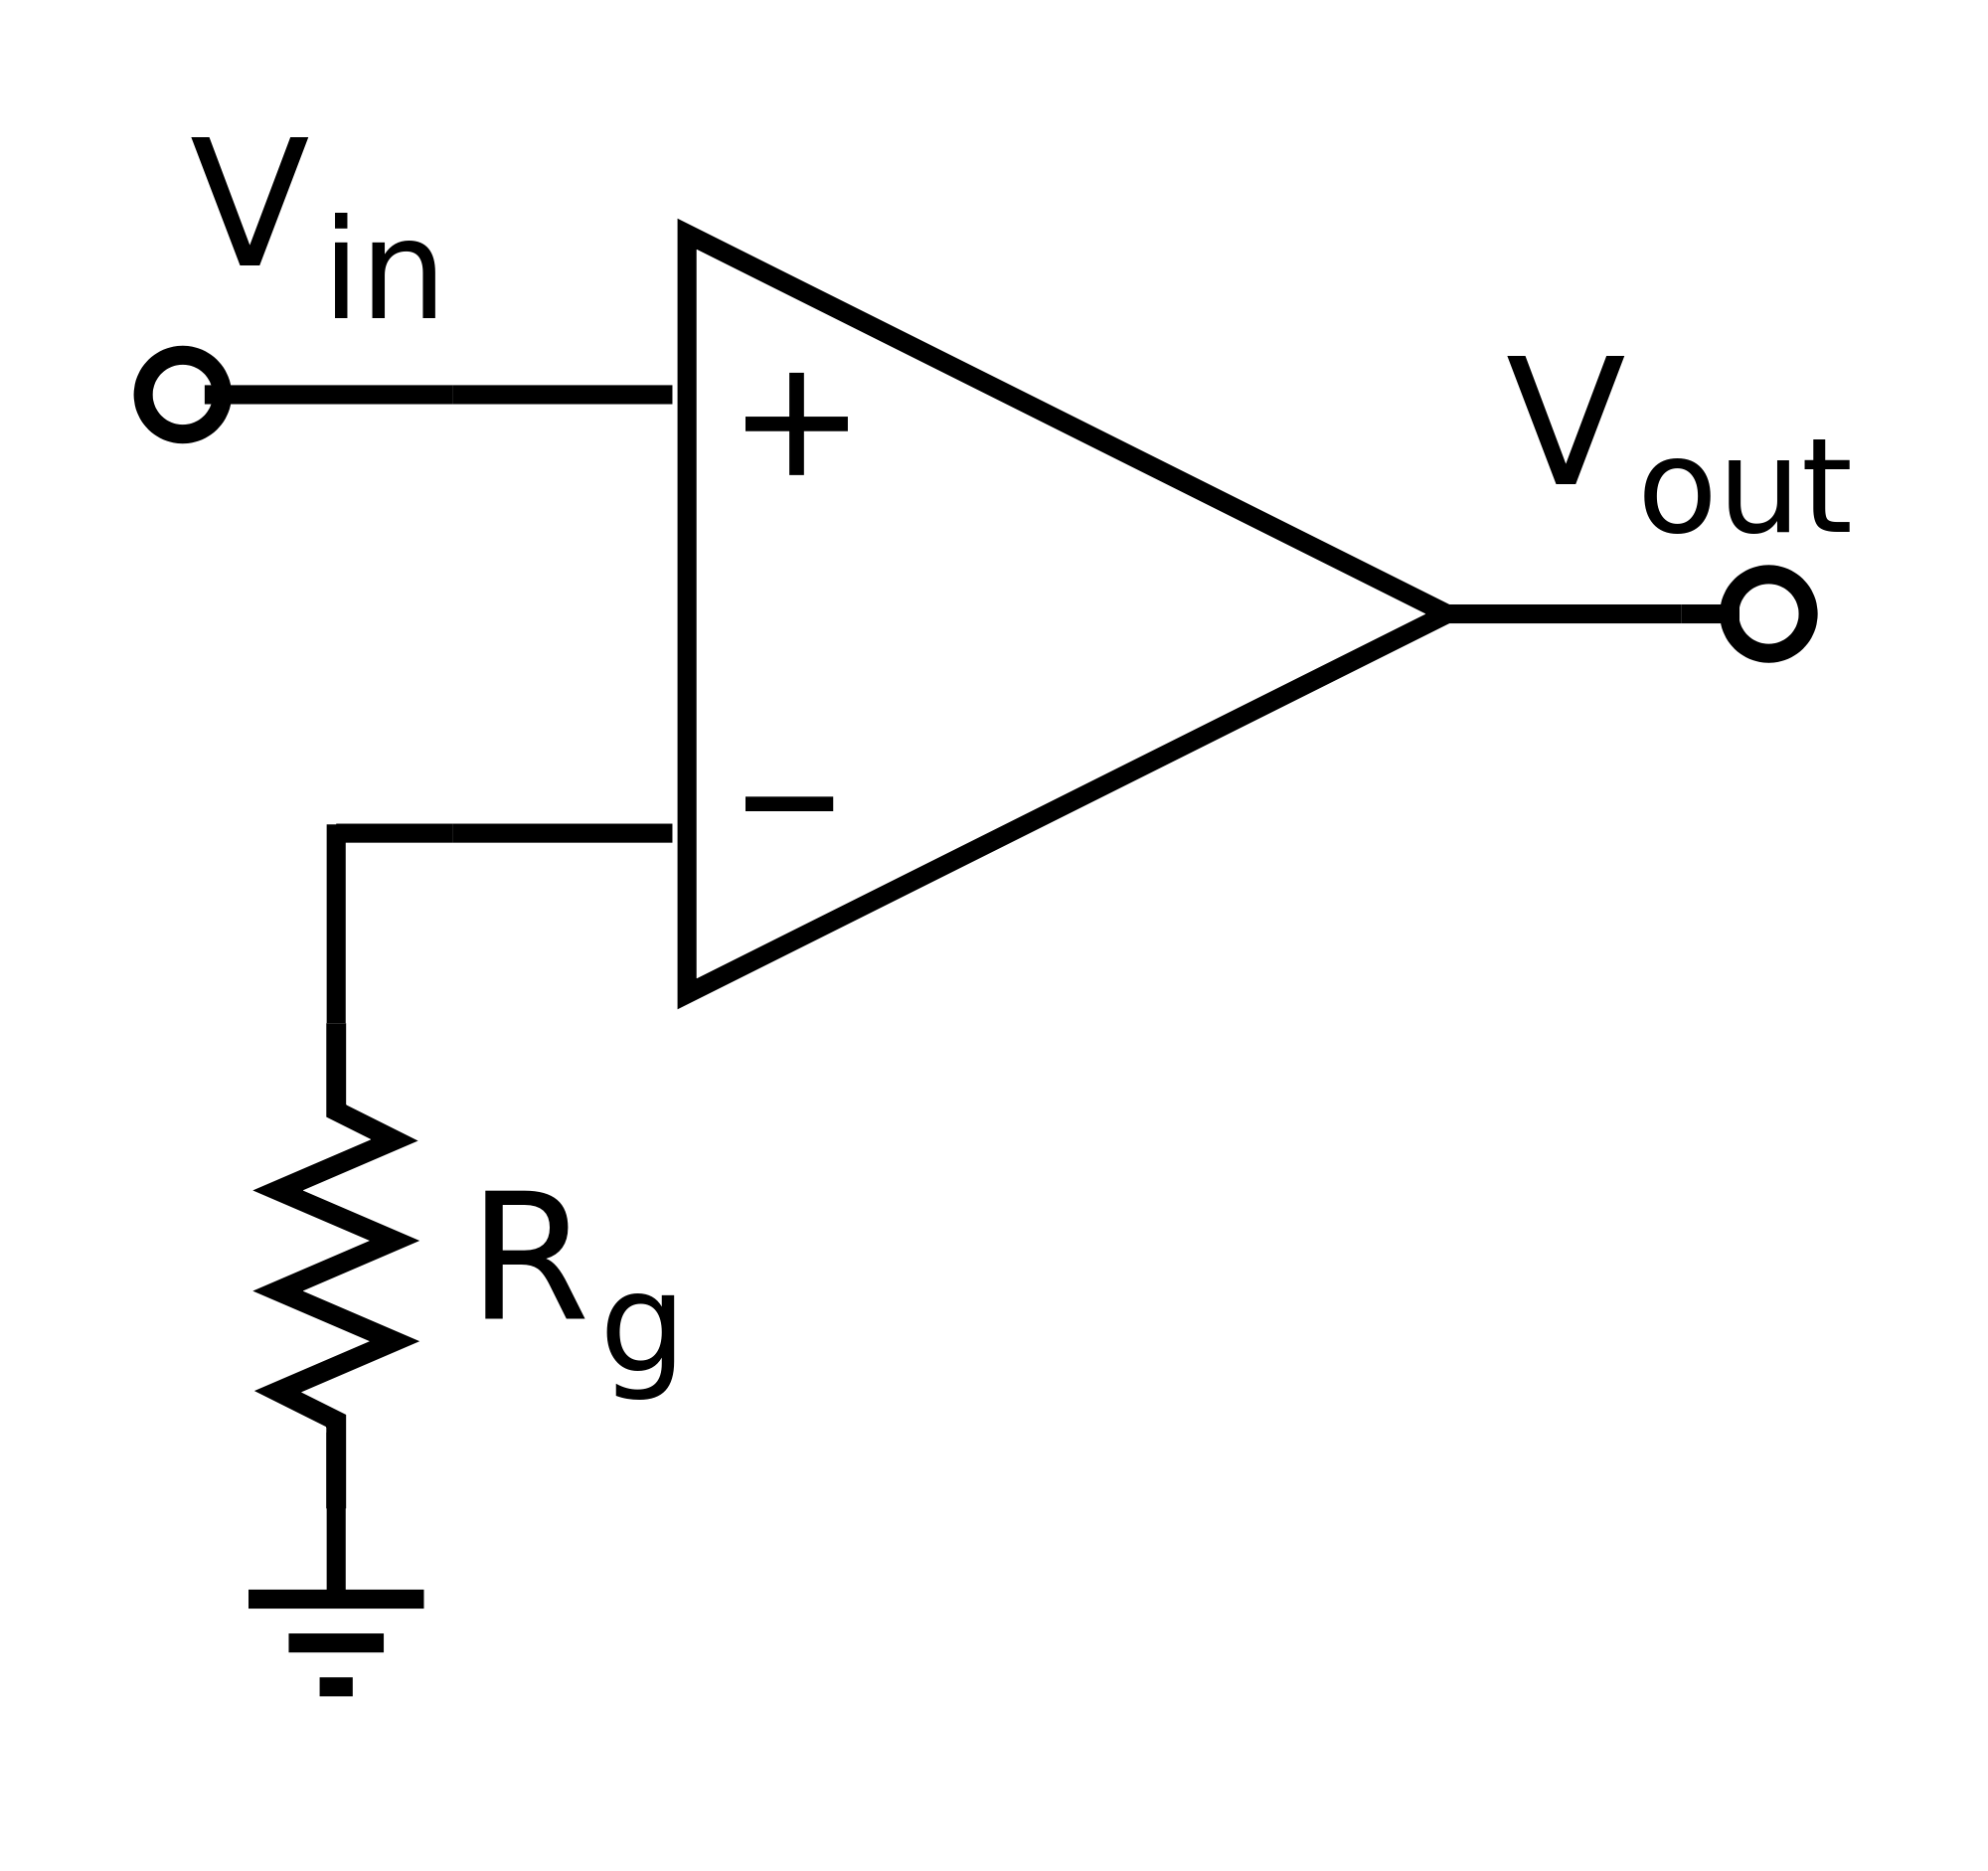
\includegraphics[width=5.6cm]{./bilder/OP-förstärkare.png}
\end{textblock*}


\subsection*{Jag drikker Tuborg} 
\index[alfa]{Jag drikker Tuborg}
\index[anfa]{Jag drikker Tuborg}
\songinfo{Synge på dansk}

\begin{parse lines}[\noindent]{#1\\}
    Jeg drikker Tuborg
    og snapser gammeldansk
    Det ær alt jeg vil,
    det ær alt jeg kan
    Jeg drikker Tuborg
    og snapser gammeldansk
    Det ær alt jeg vil og kan,
    så hold kæft jeg ær lykkelig!
\end{parse lines}

\subsection*{Alla är söta} 
\index[alfa]{Alla är söta}
\index[anfa]{Alla på eko}
%\songinfo{}

\begin{parse lines}[\noindent]{#1\\}

    Alla på eko,
    har koll på vårt klimat
    Utan dom får vi förgiftad mat
    Och dom på eko,
    älskar alla djur
    och det tycker vi är tur,
    för dom är så söta   
\end{parse lines}

\newpage

\subsection*{Måsen} 
\index[alfa]{Måsen}
\index[anfa]{Det satt en mås på en klyvarbom}
\songinfo{Mel: När månen vandrar}

\begin{parse lines}[\noindent]{#1\\}
    Det satt en mås på en klyvarbom,
    och tom i krävan var kräket
    Och tungan lådde i skeppar'ns gom,
    där han satt uti bleket
    Jag vill ha sill hördes måsen rope,
    och skeppar'n svarte: Jag vill ha OP,
    om blott jag får, om blott jag får
    
    Nu lyfter måsen från klyvarbom,
    och vinden spelar i tågen
    OP:n svalkat har skeppar'ns gom,
    jag önskar blott att jag såg 'en
    Så nöjd och lycklig, den arme saten,
    han sätter storsegel den krabaten
    Till sjöss han far, och halvan tar
    
    Den mås som satt på en klyvarbom,
    den är nu död och begraven
    Och skeppar'n som drack en flaska rom,
    han har nu drunknat i haven
    Så kan det gå om man fått för mycke',
    om man för brännvin har fattat tycke
    Vi som har kvar, vi resten tar
    
\end{parse lines}

\newpage

\subsection*{Musen} 
\index[alfa]{Musen}
\index[anfa]{Det satt en mus i en hushållsost}
%\songinfo{}

\begin{parse lines}[\noindent]{#1\\}
    Det satt en mus i en hushållsost,
    Och åt och åt utan måtta
    Tills osten blivit en mushåls-ost,
    och han en klotformad råtta
    "Så bra", sa musen, "att va en fettboll,
    nu kan jag rulla med hast åt rätt håll:
    Ostindien! Ostindien!"
\end{parse lines}

\subsection*{Moosen} 
\index[alfa]{Moosen}
\index[anfa]{Det satt en älg i en klyvartopp}
%\songinfo{}
\begin{parse lines}[\noindent]{#1\\}
    Det satt en älg i en klyvartopp,
    förklädd i älgjaktens månad
    Han var befjädrad till horn och kropp,
    och skepparn blev smått förvånad
    "Jag är en mås, goa skepparn" ljög den
    förklädda älgen, därefter flög den
    Mjukt föll han sen,
    på skepparen
\end{parse lines}

\subsection*{Mesen} 
\index[alfa]{Mesen}
\index[anfa]{Det satt en mes i en klyvarmast}
%\songinfo{}

\begin{parse lines}[\noindent]{#1\\}
    Det satt en mes i en klyvarmast,
    där sågs han ragla och svaja
    För trots att frön var hans enda last,
    var han full som en kaja
    "Vad har du gjort!" hördes skepparn stöna,
    och mesen svarte "Jag rökte fröna,
    i egen holk, i egen holk"
\end{parse lines}

\newpage

\subsection*{Boten} 
\index[alfa]{Boten}
\index[anfa]{Min kompis Anna, hon är en bot}
%\songinfo{}

\begin{parse lines}[\noindent]{#1\\}
    Min kompis Anna, hon är en bot,
    hon rensar upp i kanalen
    Och varje gång jag hör hennes låt,
    så får jag ont i analen
    Jag är så trött på den jävla låten,
    kan någon vänlig själ banna boten?
    Jag vete fan, jag fick en ban
\end{parse lines}

\subsection*{Kompistipset} 
\index[alfa]{Kompistipset}
\index[anfa]{Min kompis Bosse, en bigamist}
%\songinfo{}

\begin{parse lines}[\noindent]{#1\\}
    Min kompis Bosse, en bigamist,
    tar alltid två öl i baren
    Han säger "Allting kan verka trist,
    ifall man blott bara tar en
    Nej, ta och skaffa dig en till fru och
    be alltid bartendern om en duo
    Så skål min vän, och skål igen!"
\end{parse lines}

\subsection*{När månen vandrar} 
\index[alfa]{När månen vandrar}
\index[anfa]{När månen vandrar sin tysta ban}
%\songinfo{}

\begin{parse lines}[\noindent]{#1\\}
    När månen vandrar sin tysta ban
    och tittar in genom rutan
    Då tänker jag, att på ljusan da'n,
    då kan jag klara mig utan
    Då kan jag klara mig utan måne,
    men utan Renat och utan Skåne?
    Det vete fan, det vete fan    
\end{parse lines}

\newpage

\subsection*{När måsen vandrar} 
\index[alfa]{När måsen vandrar}
\index[anfa]{Om du en sittning vill sakta ner}
%\songinfo{}

\begin{parse lines}[\noindent]{#1\\}
    Om du en sittning vill sakta ner 
    och alla gästerna störa 
    Ja, då räcker det att de ser, 
    att de nu måsen ska köra 
    Den jävla låten, den är så tråkig 
    “Men den här texten är inte pjåkig” 
    Den åker ut 
    Så håll din trut
\end{parse lines}

\subsection*{JAS:en} 
\index[alfa]{JAS:en}
\index[anfa]{Där flög en JAS över Västerbron}
%\songinfo{}

\begin{parse lines}[\noindent]{#1\\}
    Där flög en JAS över Västerbron,
    men styrsystemet var trasigt
    Piloten sköt ut sig med kanon,
    för planet svängde så knasigt
    "Jag vill ju uppåt, jag vill ju mer"
    Men planet svarte: "Jag vill ju ner,
    mot alla hjon, på Västerbron" 
\end{parse lines}


\begin{textblock*}{10cm}(0.0cm, 0.5cm) % {width}(x, y)
    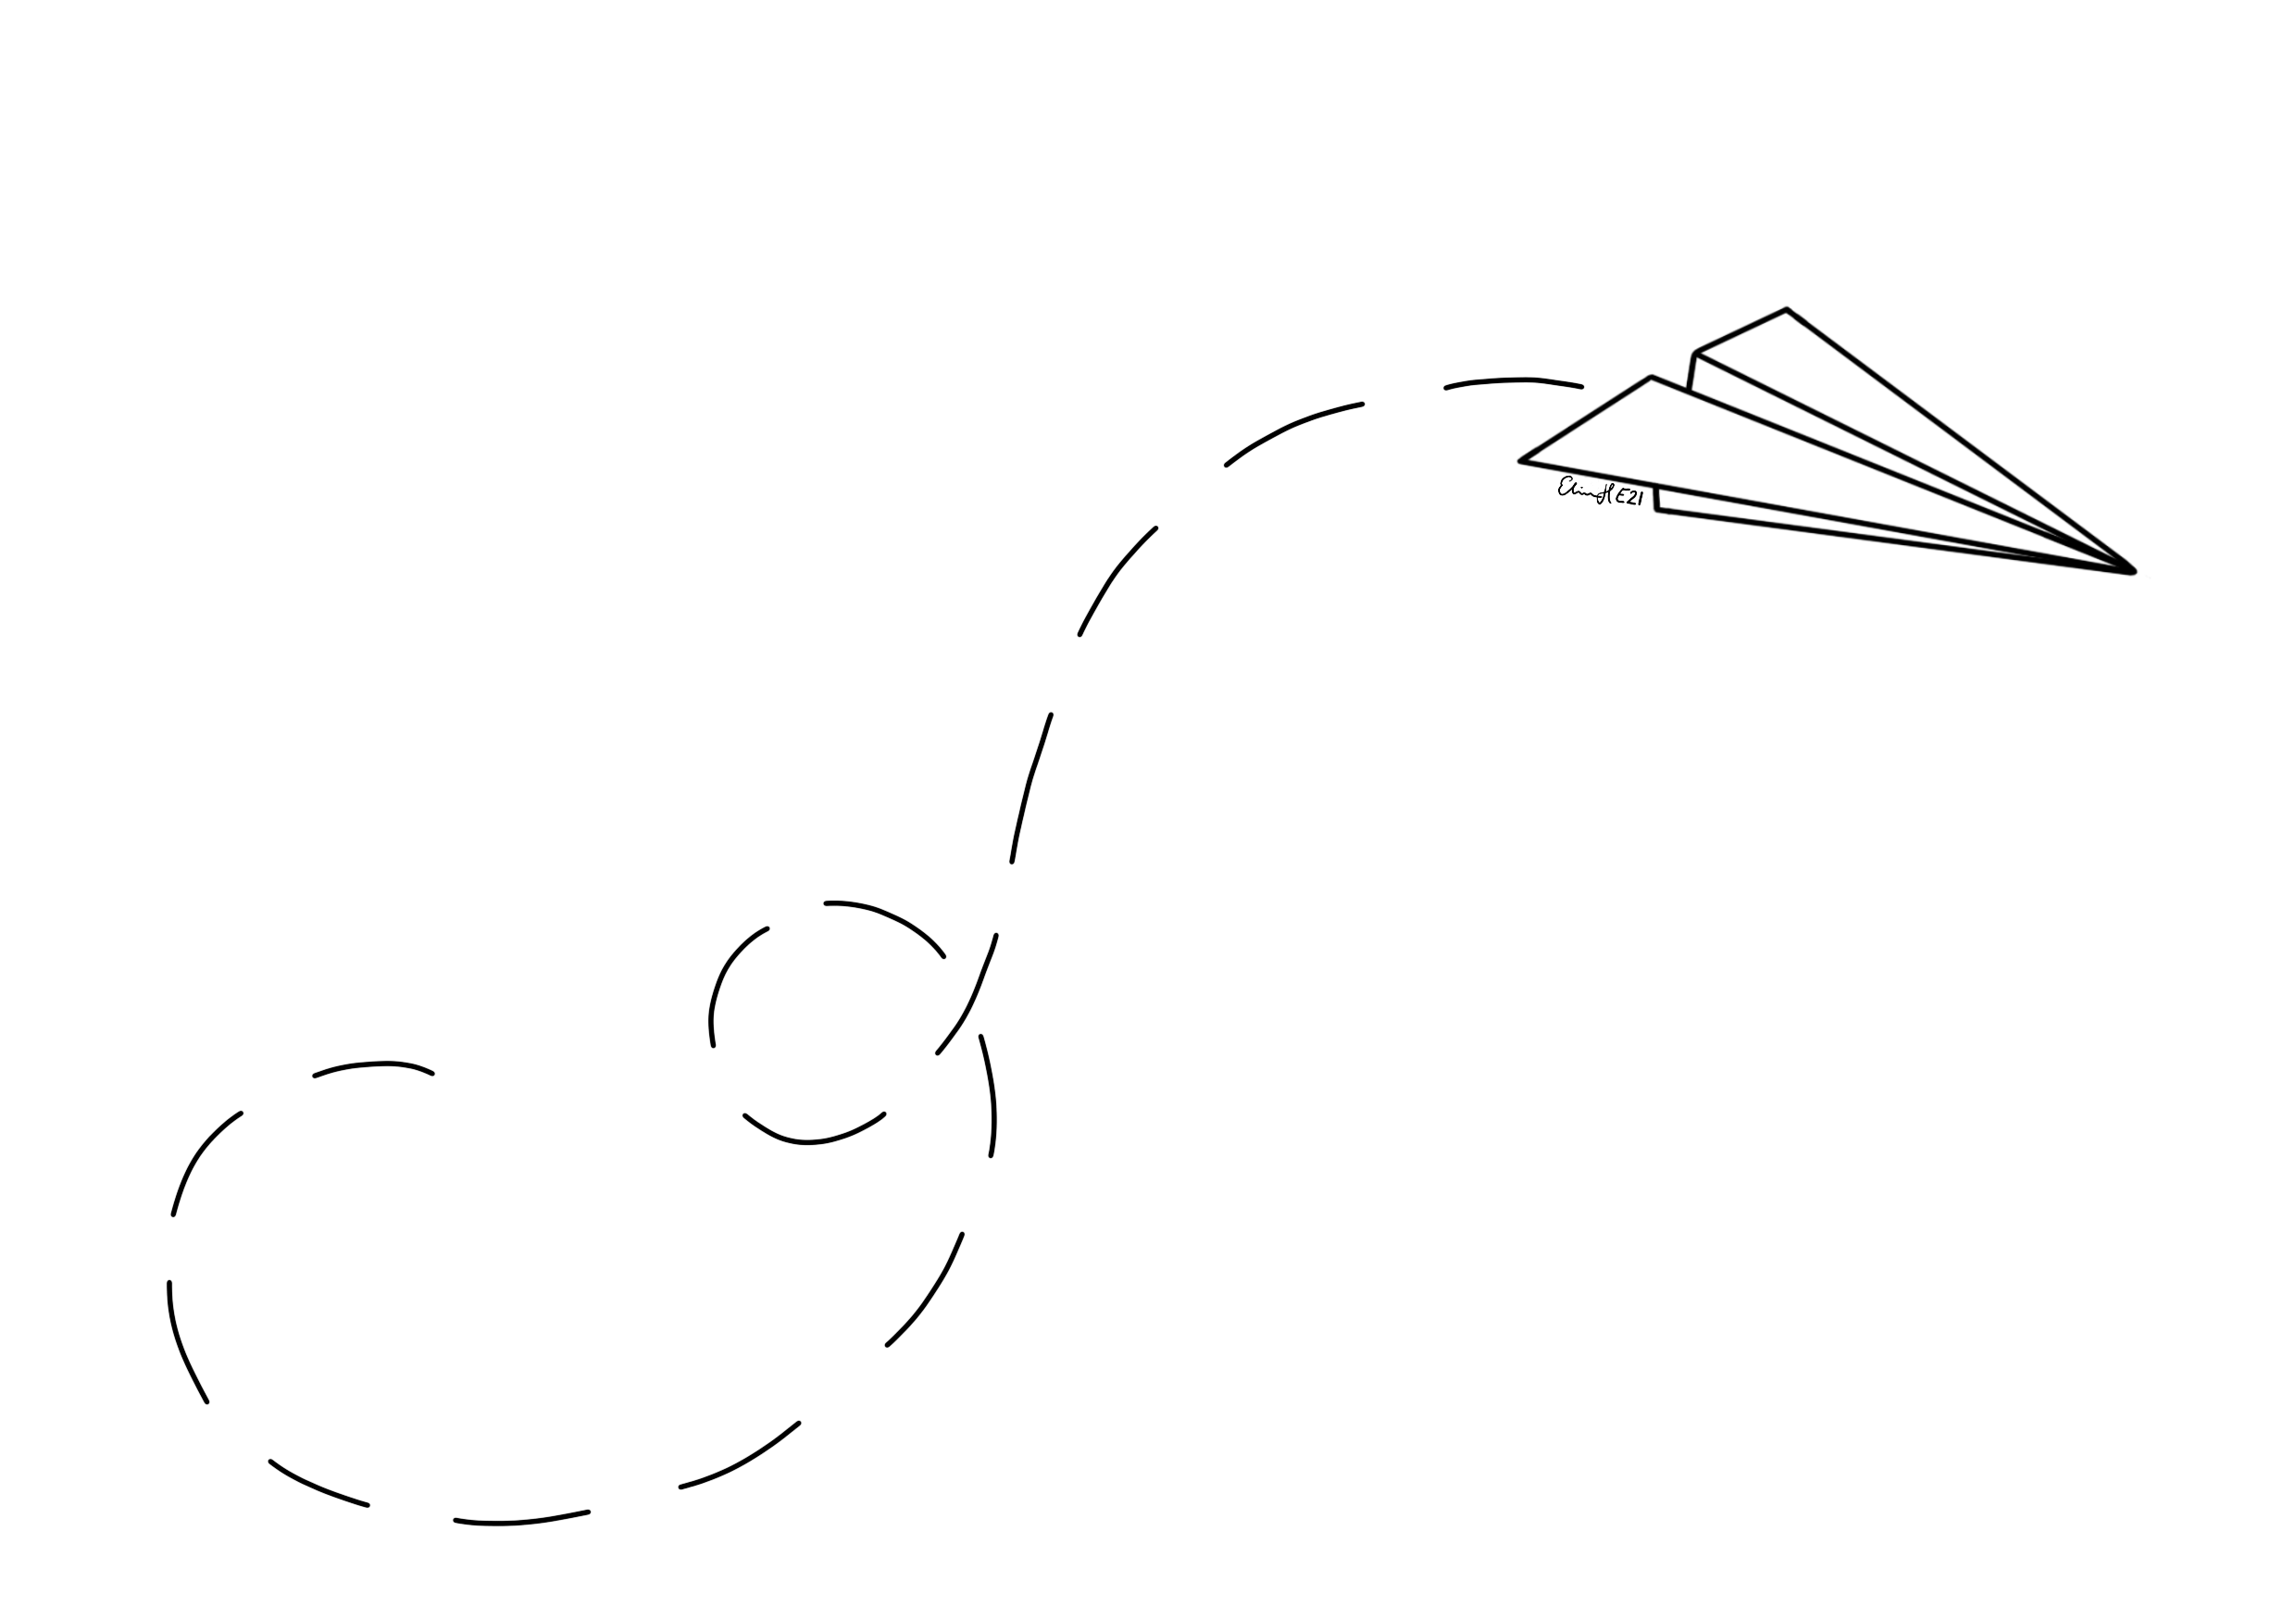
\includegraphics[width=20cm]{./bilder/pappersplan_signerad.png}
\end{textblock*}

\newpage
\noBackground

\begin{comment}
\begin{textblock*}{10cm}(1.0cm, 1.0cm) % {width}(x, y)
    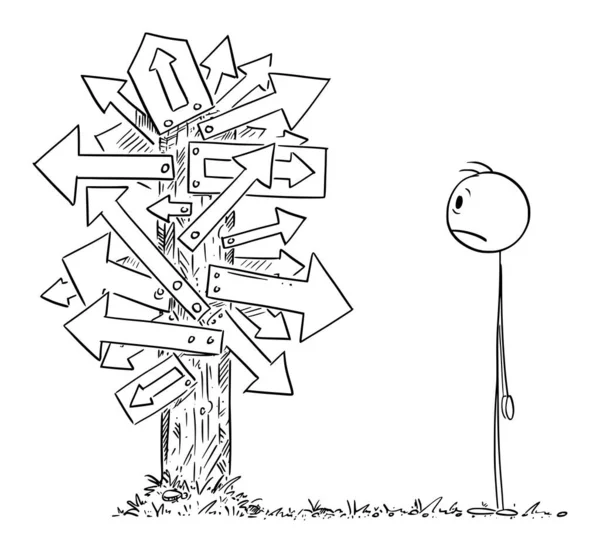
\includegraphics[width=20cm]{./bilder/roda_havet_test.png}
\end{textblock*}

\vspace*{5cm}
\end{comment}

\begin{textblock*}{10cm}(-10.3cm, 0.3cm) % {width}(x, y)
    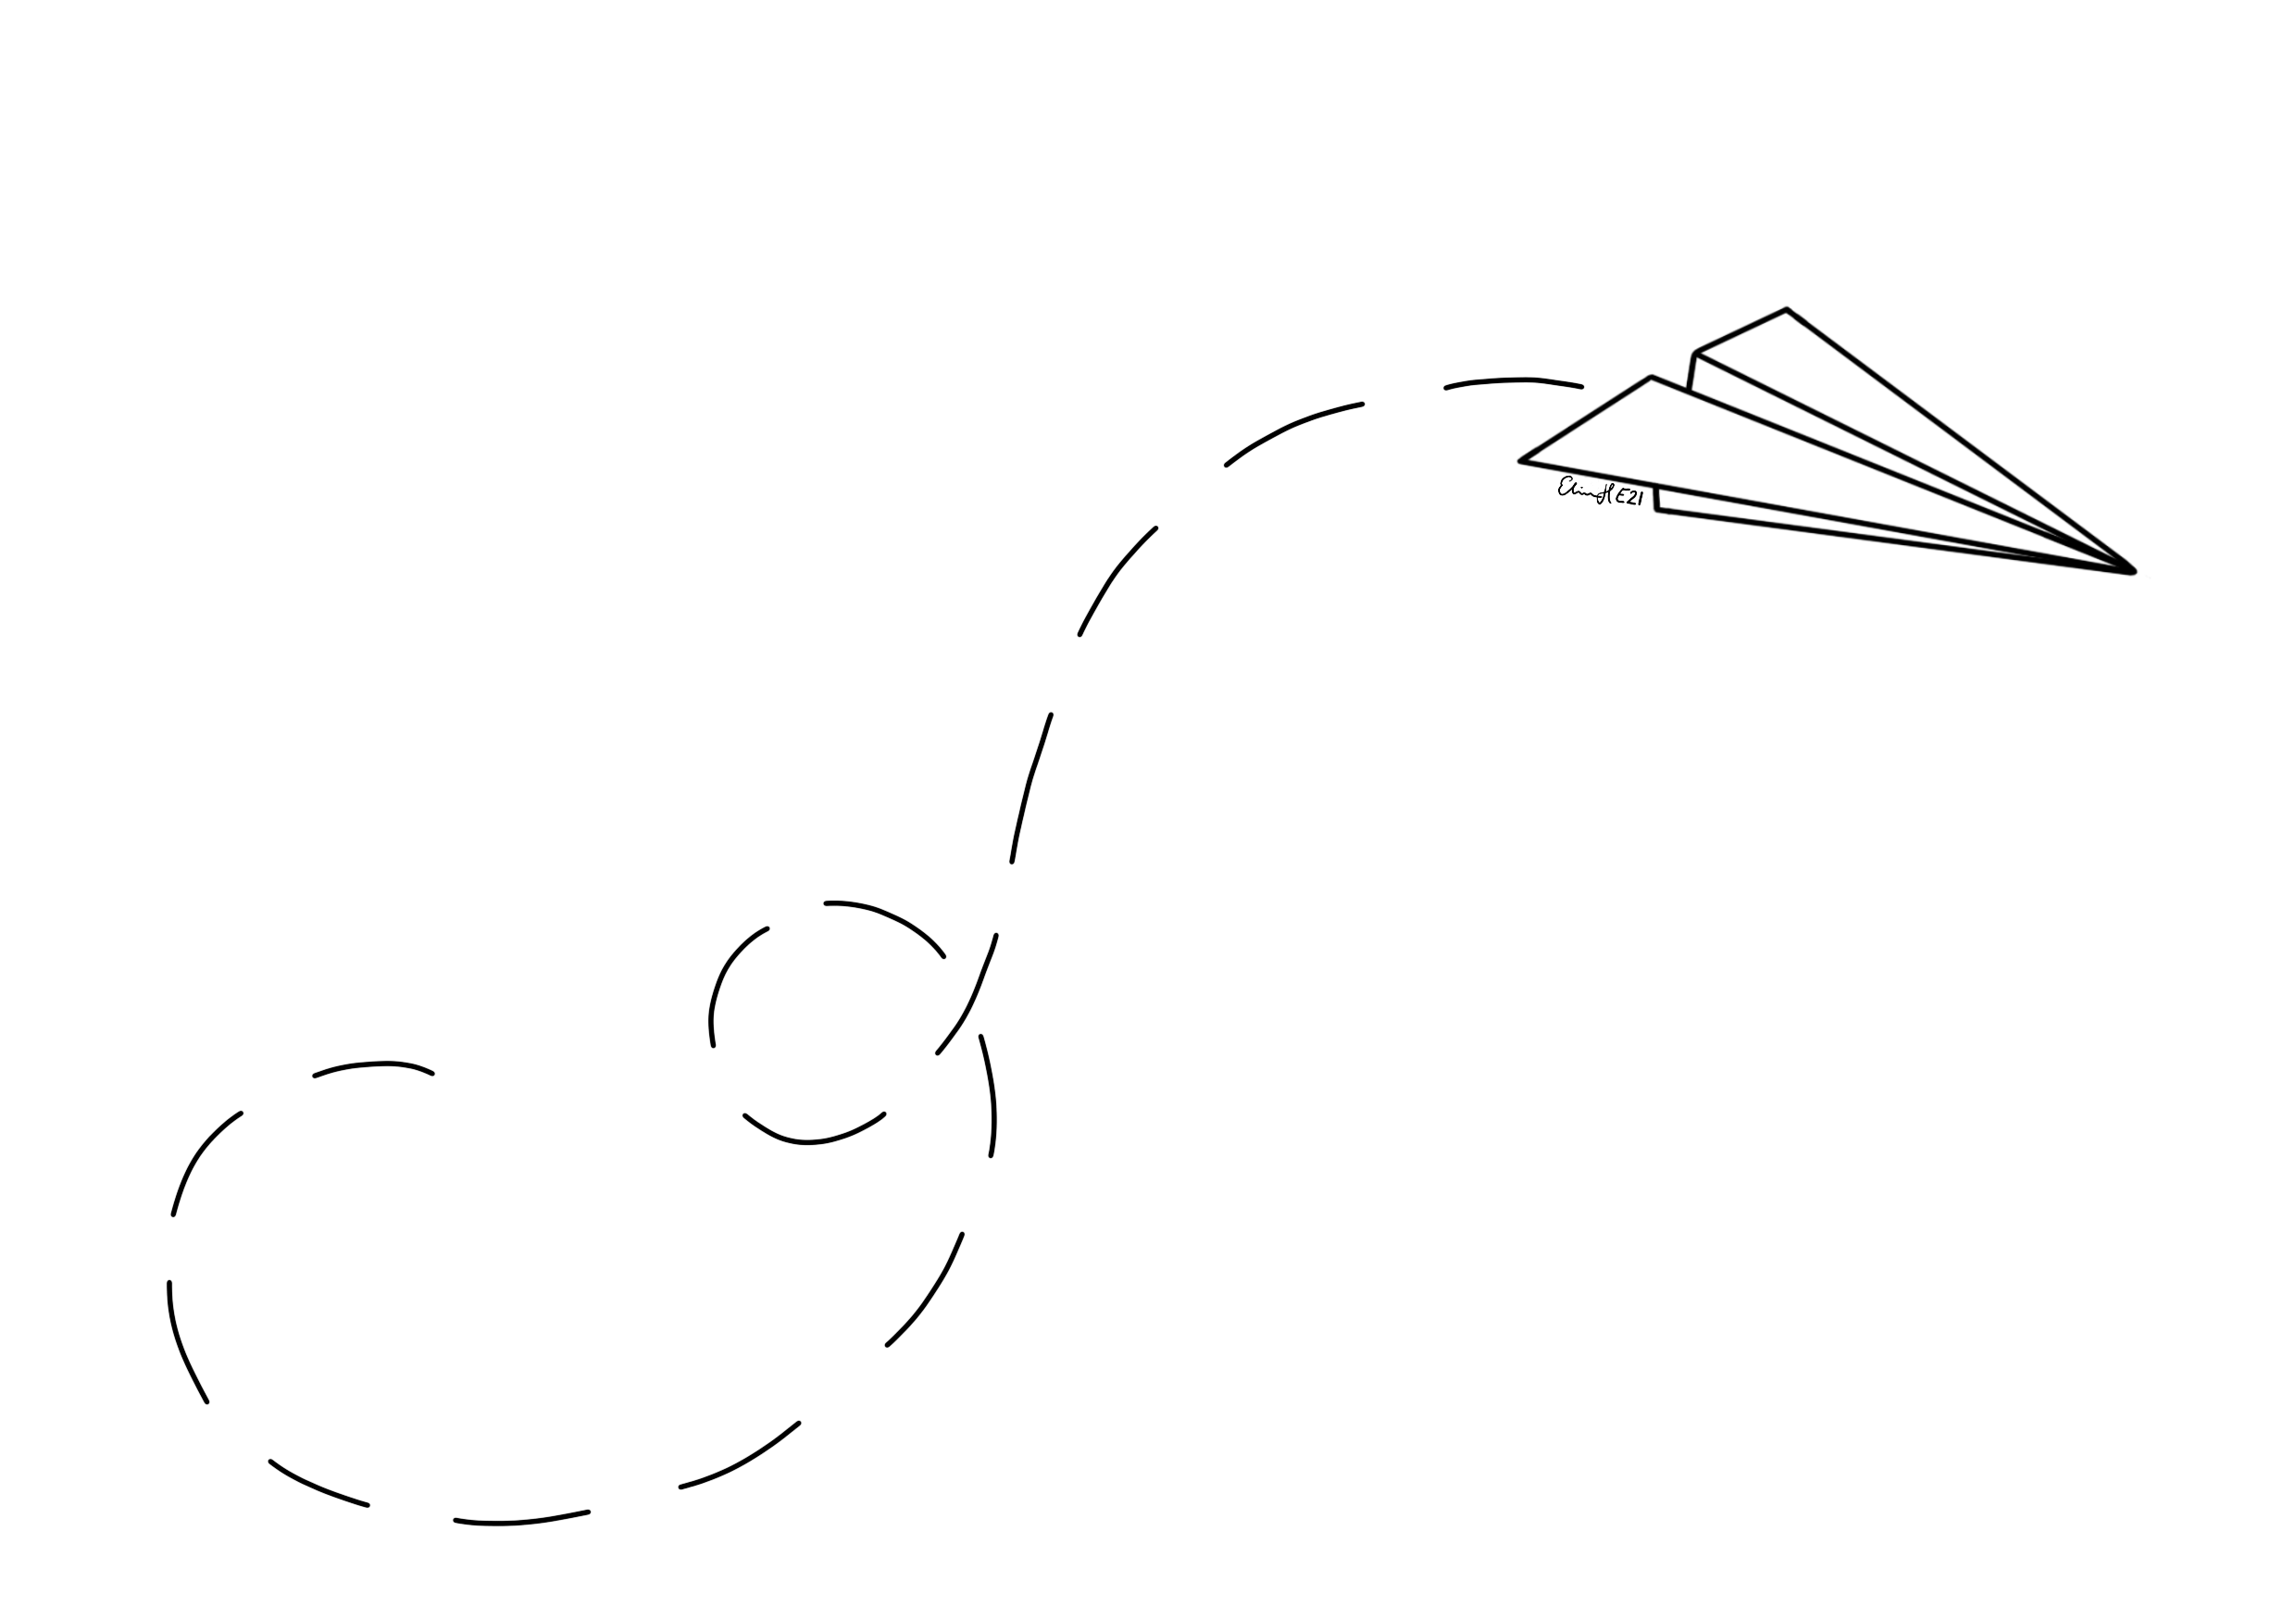
\includegraphics[width=20cm]{./bilder/pappersplan_signerad.png}
\end{textblock*}

\vspace*{5cm}
\subsection*{Röda havet} 
\index[alfa]{Röda havet}
\index[anfa]{Vi gingo ner till Röda havet}
\songinfo{Mel: Skrattvisa ur Orfeus i underjorden \\(Pour séduire Alcmène a la fière)}

\begin{parse lines}[\noindent]{#1\\}
    Vi gingo ned till Röda havet
    Vi lågo i där minst en kvart,
    ja, minst en kvart
    Men inte blev vi röda av 'et,
    men Röda havet det blev svart
    
    Men utav aqvavit,
    människan till kropp och själ,
    blir oskuldsfull och vit
    Men utav aqvavit,
    människan till kropp och själ,
    blir oskuldsfull och vit
\end{parse lines}

\newpage
\resetBackground

\subsection*{Stadsparksdammen} 
\index[alfa]{Stadsparksdammen}
\index[anfa]{Vi gingo ner till stadsparksdammen}
%\songinfo{}

\begin{parse lines}[\noindent]{#1\\}

    Vi gingo ner till stadsparksdammen
    Vi lågo i där minst en kvart,
    ja, minst en kvart
    Men inte blev vi av med skammen,
    men stadsparksdammen den blev svart
    
    Men utav aqvavit…

\end{parse lines}

\subsection*{Lommabukten} 
\index[alfa]{Lommabukten}
\index[anfa]{Vi gingo ned till Lommabukten}
%\songinfo{}

\begin{parse lines}[\noindent]{#1\\}

    Vi gingo ned till Lommabukten
    Vi lågo i där minst en kvart,
    ja, minst en kvart
    Men inte blev vi av med lukten,
    men Lommabukten den blev svart
    
    Men utav aqvavit...
\end{parse lines}

\newpage

\subsection*{Finska viken} 
\index[alfa]{Finska viken}
\index[anfa]{Vi gingo ner till Finska viken}
%\songinfo{}

\begin{parse lines}[\noindent]{#1\\}

    Vi gingo ner till Finska viken
    Vi lågo i där minst en kvart,
    ja, minst en kvart
    Men inte blev vi av med skiten,
    men Finska viken den blev svart
    
    Men utav aqvavit…

\end{parse lines}

\subsection*{Systembolaget} 
\index[alfa]{Systembolaget}
\index[anfa]{Vi gingo ner till Systembolaget}
%\songinfo{}

\begin{parse lines}[\noindent]{#1\\}

    Vi gingo ner till Systembolaget
    Vi stod i kö där minst en kvart,
    ja, minst en kvart
    Men inte blev vi fulla av det,
    systembolaget det gick back
    
    Men utav aqvavit…
\end{parse lines}

\vissteduatt{Visste du att aqvavit = aqua vitae = livets vatten?}
\newpage

\subsection*{Labblokalen} 
\index[alfa]{Labblokalen}
\index[anfa]{Vi gingo ned till labblokalen}
%\songinfo{}

\begin{parse lines}[\noindent]{#1\\}

    Vi gingo ned till labblokalen
    Vi var där inne minst en kvart,
    ja, minst en kvart
    Men inte blev vi av med kvalen,
    men labblokalen den blev svart
    
    Men utav aqvavit...
\end{parse lines}

\subsection*{Vi gingo ner till Edekvata} 
\index[alfa]{Vi gingo ner till Edekvata}
\index[anfa]{Vi gingo ner till Edekvata}
%\songinfo{}

\begin{parse lines}[\noindent]{#1\\}

    Vi gingo ner till Edekvata
    Vi olja borden minst en kvart,
    ja, minst en kvart
    Men manualen den vi rata,
    så Edekvata det blev svart
    
    Men utav aqvavit…
    
\end{parse lines}

\vissteduatt{Visste du att det brann i Edekvata 2010?
\\En trasa med linolja självantände...}
\newpage

\subsection*{Karnevalen} 
\index[alfa]{Karnevalen}
\index[anfa]{Vi gingo ner till karnevalen}
%\songinfo{}

\begin{parse lines}[\noindent]{#1\\}
    
    Vi gingo ner till karnevalen
    och stod i kö där minst en kvart,
    ja, minst en kvart
    Vi ville in i AF-salen,
    men inte fan kom vi nå'n vart

    För utav kösystem,
    blir det bara skit och massa allmänna problem
    För utav kösystem,
    blir det bara skit och massa allmänna problem
    
    Och vi kom fram till kravallstaketet
    och stod kvar där minst en kvart,
    ja, minst en kvart
    Sen vi var fast i köhelvetet,
    så inte fan kom vi nå'n vart
    
    För utav kösystem…
    
\end{parse lines}


\newpage
